\section{Objectives and Activities}

The project targets to evaluate the scalability of the two kind of compositions explained above. To make this evaluation, we first needed a composition to evaluate. Thus we designed a synthetical orchestration in witch each partner is another synthetical orchestration, recursively, the second's partners are also orchestrated services, until the last specific composition. The topology generated from this design is a tree, in witch each node (first kind of orchestrated service) have a pre-defined number of children. The depth of the tree is also predefined. The message received in the root node is propagated through it's children until it reaches the leaf node (the second kind of service on the process). When the leaf node receives the message, it starts the travel back to the root, whom will reply it to the client.

This tree is a choreography of orchestrated services: each node and it's children are the orchestration and the entire process is a choreography.

\subsection{Composition Generator}
To generate all this structure, we first developed ``hardcoded'' orchestrations, with NetBeans, to simulate the desired tree. When we accomplished this first task, we created a simple ruby script which generated the tree and, also, for each node of the tree, a set of WSDL and BPEL files corresponding to the service of that node.

Later we needed a way an automate way to deploy all those services on different machines, so we attached some more code on the ruby script to allocate instances of Amazon EC2 for each node of the tree. At this moment the code was starting to get ugly. It was time for some code refactoring.

After spending some time to make the code more readable, we decided to make the deploy of the process in the instances of the EC2. But NetBeans, used until this point to run the process generated, was not able to run properly from the shell, which is the only native interface with EC2 instances. After some research upon open source engines, we discovered PEtALS ESB, which have the simplest install and setup process between all the servers researched, this was the most essential feature to build the automated process.

Nowadays the script generates the tree, instantiate virtual machines on Amazon EC2, create the compositions, configure each instance to become a node of PEtALS Bus, start PEtALS server in each node and deploy the services on the ESB. This process is parallelized for each node, and the steps of the process can be followed in the shell's standard output, as shown in Figure \ref{generation-output}


\begin{figure}[htb]
	\centering
	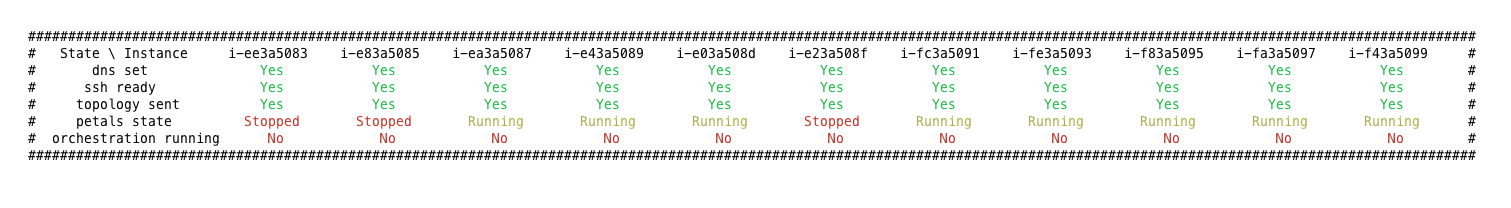
\includegraphics[trim= 10mm 0mm 10mm 0mm, clip, width=\textwidth]{images/generation-output}
	\caption{Example output from running the generator script for a tree with depth of 1 and 10 children per node}
	\label{generation-output}
\end{figure}

When it's finished, the generator outputs the host of the process (\emph{Public DNS} of Root Node), from which port it is reachable, the path to the service and the id of this root node (to compose the SOAP messages).

\subsection{Message Sender}

In order to evaluate the responses of the synthetical compositions, we needed another Ruby script that sends messages of $S$ sizes and with a frequency of $F$ messages per seconds.

Given the fact that the connection with the Cloud is very unstable, we added a fourth parameter to define how many times the batch of messages will be sent, so when there's a lot of traffic on the Net, any extraordinary case will not be representative on the overall mean. An example of execution can be found at Figure \ref{send-msg-output}


\begin{figure}[htb]
	\centering
	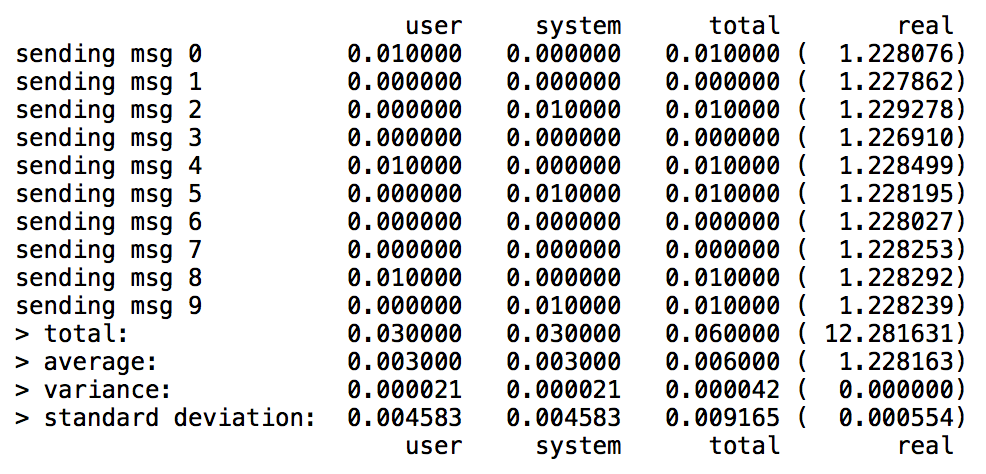
\includegraphics[width=0.8\textwidth]{images/send-msg-output}
	\caption{Example output from running the send message script with $S = 1$, $F = 1$, $BatchSize = 10$}
	\label{send-msg-output}
\end{figure}
